\begin{figure}[H]
    \centering
    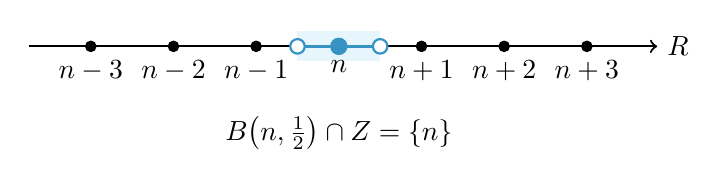
\begin{tikzpicture}[scale=1.05]
        \coordinate (n) at (0,0);
        \coordinate (a) at (-0.5,0);
        \coordinate (b) at (0.5,0);

        % Reta real contendo os pontos inteiros.
        \draw[->, thick] (-3.75,0) -- (3.85,0) node[right] {$\mathbb R$};

        % A bola aberta em R centrada em n com raio 1/2.
        \path[fill=Cerulean!10] (-0.5,-0.18) rectangle (0.5,0.18);
        \draw[Cerulean!80!black, very thick] (a) -- (b);
        \filldraw[fill=white, draw=Cerulean!80!black, thick] (a) circle (2.5pt);
        \filldraw[fill=white, draw=Cerulean!80!black, thick] (b) circle (2.5pt);

        % Pontos de Z ao redor de n.
        \foreach \x/\rotulo in {-3/{n-3},-2/{n-2},-1/{n-1},1/{n+1},2/{n+2},3/{n+3}} {
            \filldraw[black] (\x,0) circle (1.8pt);
            \node[below] at (\x,-0.05) {$\rotulo$};
        }

        % O ponto n fica isolado dentro da bola escolhida.
        \filldraw[Cerulean!80!black] (n) circle (2.8pt);
        \node[below] at (0,-0.05) {$n$};
        \node[black] at (0,-1.05)
            {$B\!\left(n,\frac12\right)\cap\mathbb Z=\{n\}$};
    \end{tikzpicture}
    \caption{Cada ponto $n\in\mathbb Z$ é isolado em $\mathbb Z$.}
    \label{fig:pontoIsoladoZ}
\end{figure}
